\documentclass[11pt, letterpaper, twoside]{article}
\usepackage[letterpaper, portrait, left=1in, right=1in, top=1in, bottom=1in]{geometry}\usepackage{amsmath}
\usepackage{amssymb}
\usepackage{graphicx}
\usepackage[explicit]{titlesec}
\usepackage{epstopdf}
\usepackage{amsmath}
\usepackage{inputenc}
\usepackage{enumitem}
\usepackage{booktabs, multirow} %for borders and merged ranges
\usepackage{soul}% for underlines
\usepackage[table]{xcolor} % for cell colors
\newcommand\aug{\fboxsep=-\fboxrule\!\!\!\fbox{\strut}\!\!\!} %Use \aug to make a equal column for an augmented matrix. Ie. 1 & 2 & 3 & 4 & \aug & x \\
\begin{document}
\begin{titlepage}
\centering
\vspace*{60px}
\hspace{0pt}

\includegraphics[width=0.2\textwidth]{logo}\par\vspace{1cm}
{\scshape\LARGE Athabasca University \par}
\vspace{1cm}
{\scshape\Large MATH 265\par}
\vspace{1.5cm}
{\huge\bfseries Assignment 4\par}
\vspace{2cm}
{\Large\itshape Stanley Zheng\par}
\vfill
{\large September 3, 2020\par}
\vspace*{50px}
\hspace{0pt}
\pagebreak
\end{titlepage}
\begin{enumerate}
\item 
\begin{enumerate}[label=\alph*)]
\item ‌‌ 

\vspace{0.2cm}
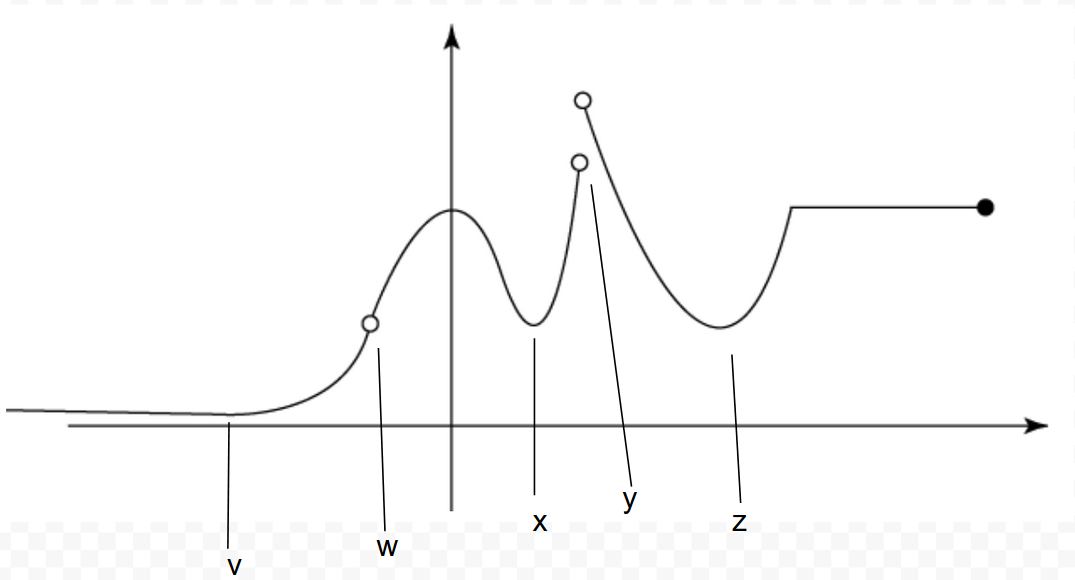
\includegraphics[width=0.7\textwidth]{q1}\par

The domain of the function \(g\) is \((-\infty, w)\cup(w, x)\cup(x, y]\)
\item The function \(g\) is continuous from \((-\infty, w)\cup(w, x)\cup(x, y]\).
\item The local maximum ix at \(x=0\), since the derivative is 0.
\item The local minimum is at two points, \(x\) and \(z\), where the derivative is zero.
\item There is no absolute maximum as the derivative at \(y\) is undefined, and \(y\) is not included in the domain.
\item The absolute minimum is at \(v\). It appears as though the graph has negative slope as \(x\) decreases beyond \(v\) to infinity.
\end{enumerate}
\item %q2

\item %q3

\item %q4
First, we need to find relative distances for swimming and jogging.
Let's let \(\angle PWE\) be \(\theta\).
We can create a triangle by connecting points \(PWE\) with straight lines.
We know from Thale's theorem that an angle inscribed across the diameter of a circle is always \(90^\circ\), so this triangle is a right triangle.
Then, the swimming distance, line \(PW\), is \(3\cos\theta\).
The arc length for jogging is \(\theta r\), and our diameter is 3km, so the jogging distance is \(2\cdot1.5\theta\). 
We must multiply by 2 since the angle is not measured at the center of the circle, but rather subtends it.

We know that critical points are found where the derivative of a function is 0 or undefined.
To find the derivative, we can find an equation for the time of the journey, then differentiate.

\[\frac{1}{24}\cdot3\theta+\frac{1}{3}\cdot3\cos\theta\]
\[\frac{\theta}{8}+\cos\theta\]

We can then differentiate and find zeros.
\[0=\frac{1}{8}-\sin\theta\]
\[\sin\theta=\frac{1}{8}\]
\[\sin^{-1}\left(\frac{1}{8}\right)=\theta\]
We have \(\theta\approx0.125\). 
To find the distance to jog, we multiply by 3.
The final distance Peter should jog to arrive at point W in the least amount of time is \(\boxed{0.376\text{km}}\)

\item %q5

\item %q6



\end{enumerate}
\end{document}